\RequirePackage[l2tabu, orthodox]{nag}
\RequirePackage{silence}
\documentclass[french,english]{beamer}
\input{preamble/packages}
\input{preamble/math_basics}
\input{preamble/math_mine}
\input{preamble/redac}
\input{preamble/draw}
\input{preamble/acronyms}

\sisetup{retain-explicit-plus}

%\setbeamertemplate{headline}[singleline]
%\setbeamertemplate{footline}[authortitle]

\title{Reasons and Means to Model Preferences as Incomplete}
\subject{Preference modeling}
\keywords{MCDA, MCDM, preference models, partial orders}
\author[Olivier Cailloux]{\emph{Olivier Cailloux}\inst{1} \and Sébastien Destercke\inst{2}}
\institute[LAMSADE]{\inst{1} LAMSADE, Université Paris-Dauphine \and \inst{2} Heudiasyc, Université de Technologie de Compiègne}
\date{\formatdate{6}{10}{2017}}

\begin{document}
\begin{frame}[plain]
	\tikz[remember picture,overlay]{
		\path (current page.south west) node[anchor=south west, inner sep=0] {
			\includegraphics[height=1cm]{LAMSADE95.jpg}
		};
		\path (current page.south) ++ (0, 1mm) node[anchor=south, inner sep=0] { 
			\includegraphics[height=9mm]{Dauphine.jpg}
		};
		\path (current page.south east) node[anchor=south east, inner sep=0] {
			\includegraphics[height=1cm]{PSL.png}
		};
		\path (current page.south) ++ (0, 4em) node[anchor=south, inner sep=0] {
			\scriptsize\url{https://github.com/oliviercailloux/Survey-pref-models-pres}
		};
%thanks to https://stackoverflow.com/questions/2423777/is-it-possible-to-create-a-remote-repo-on-github-from-the-cli-without-opening-br/13366414#13366414
%curl -u 'oliviercailloux' https://api.github.com/user/repos -d '{"name":"Survey-pref-models-pres"}'
%git remote add origin git@github.com:oliviercailloux/Survey-pref-models-pres.git
%git push origin master
	}
	\titlepage
\end{frame}
\addtocounter{framenumber}{-1}

%\begin{frame}
%	\frametitle{Preliminary question}
%	choose a program to prepare against an epidemic outspring that would result otherwise in 600 deaths
%	\begin{itemize}
%		\item Compare $x$ = exactly 200 lives saved to $y$ = $1/3$ of saving all $600$ persons, and $2/3$ of saving nobody.
%	\end{itemize}
%\end{frame}

%\begin{frame}
%	\frametitle{Question}
%	Choose a program to prepare against an epidemic outspring that would result otherwise in 600 deaths
%	\begin{itemize}
%		\item Compare $p_1$ = $1/3$ of saving all $600$ persons, and $2/3$ of having all $600$ persons dying to $y$ = exactly 400 persons dying
%	\end{itemize}
%\end{frame}

\begin{frame}
	\frametitle{Outline}
	\tableofcontents[hideallsubsections, sectionstyle=shaded/show]
\end{frame}

\begin{frame}
	\frametitle{Overview}
	\begin{itemize}
		\item Why model preferences?
		\item What is a model of preferences?
		\item Then: Not the usual tutorial talk!
		\item Incomplete models in practice: a topic for research!
		\item Motivate: reasons
		\item Sketch means
		\item Illustrate on recommender systems
		\item Detour via: psychology, economy…
	\end{itemize}
	\emph{Disclaimer}: I am \emph{not} an expert of all these fields.
%	(My main expertise: preference modeling; group decision making. Other interests: social choice, epistemology.)
\end{frame}

\AtBeginSection{
	\begin{frame}
		\frametitle{Outline}
		\tableofcontents[currentsection, hideallsubsections]
	\end{frame}
}

\section[Preference models]{Preference models: what, why?}
\subsection{Models basics}
\begin{frame}
	\frametitle{\subsecname}
	\begin{itemize}
		\item A set of alternatives $\allalts$
		\item A user
		\item A binary relation of preference over $\allalts$: $R \subseteq A × A$
		\item $a R b$ iff the user perfers $a$ over $b$
		\item Strictly prefers: $R$ denoted $\succ$
		\item Weakly prefers: $R$ denoted $\succeq$
	\end{itemize}
	\begin{exampleblock}{Hotels}
		\begin{itemize}
			\item Alternatives are hotels
			\item User wants to choose an hotel
		\end{itemize}
	\end{exampleblock}
\end{frame}

\begin{frame}
	\frametitle{Extensions, remarks}
	\begin{itemize}
		\item Preference modeling interested in the \emph{decision} problem (hence vocabulary differences)
		\item Decision maker / user
		\item Alternative / object
		\item Goal is usually to select one alternative
		\item Sometimes the model includes more than one binary relation
		\item A model may also represent preference for $a$ against prototypical alternatives (4 stars hotel)
	\end{itemize}
\end{frame}

\begin{frame}
	\frametitle{Examples}
	\begin{exampleblock}{Movies}
		\begin{itemize}
			\item Alternatives are movies
			\item User wants to choose next movie to see
		\end{itemize}
	\end{exampleblock}
	\begin{exampleblock}{Students}
		\begin{itemize}
			\item Alternatives are students
			\item User is a teacher ranking students
		\end{itemize}
	\end{exampleblock}
	\begin{exampleblock}{Production site}
		\begin{itemize}
			\item Alternatives are production sites
			\item User is a CEO, wants to choose where to locate a factory
		\end{itemize}
	\end{exampleblock}
\end{frame}

\begin{frame}
	\frametitle{Recommendation system view}
	(Disclaimer: Oversimplified view!)
	\begin{exampleblock}{Movies}
		\begin{itemize}
			\item Alternatives are movies
			\item User rates movies she has seen: 1 to 5 stars
			\item The system learns to predict ratings: unseen movie, what would be its rating?
			\item The system recommends the next movie to see (one of the predicted 5 stars)
		\end{itemize}
	\end{exampleblock}
\end{frame}

\begin{frame}
	\frametitle{Link with recommendation systems}
	Link with preference model?
	\begin{itemize}
		\item $m_1 \mathrel{R} m_2$ iff [rating $m_1$] ≥ [rating $m_2$]
		\item A weak order with five equivalence classes
	\end{itemize}
	Differences?
	\begin{itemize}
		\item (Generally) many users considered simultaneously
		\item $R$ restricted to max five equivalence classes
		\item Assumes differences (5 VS 3 > 2 VS 1) are not used; no semantics to categories
	\end{itemize}
	Those (important) differences: neglected here
\end{frame}

\subsection{Why model preferences?}
\begin{frame}
	\frametitle{\subsecname}
	Two views
	\begin{block}{Descriptive}
		\begin{itemize}
			\item Preference model describes normal behavior
			\item Must predict correctly
		\end{itemize}
	\end{block}
	\begin{block}{Prescriptive}
		\begin{itemize}
			\item Preference model serves to recommend
			\item May voluntarily differ from prediction
		\end{itemize}
	\end{block}
\end{frame}

\begin{frame}
	\frametitle{Do we want to prescribe?}
	\begin{itemize}
		\item Recommender system POV: usually mainly descriptive / predictive
		\item But: User may have “normal” behavior that she rejects when thinking carefully
		\item Extreme case: user violating dominance (Choose a hotel less good on every aspects)
		\item Realistic case: user discriminates unwillingly
		\item Other examples to come
	\end{itemize}
\end{frame}

\subsection{Some preference models}
\begin{frame}
	\frametitle{Multiple criteria decision making (MCDM) context}
	\begin{itemize}
		\item Alternatives evaluated using a set of criteria $\crits$
		\item Each criterion $\crit$: evaluation scale $X_\crit$
		\item $\allalts = \prod_{\crit \in \crits} X_\crit$
		\item Model: $R$ over $\allalts$
	\end{itemize}
	\begin{center}
		\begin{tikzpicture}
			\path node[matrix of nodes, ampersand replacement=\&] (my matrix) {
					\& quantity	\& taste	\& \node[align=left] {supports\\pollinators};	\& \node[align=left] {resists\\to cold};\\
				Tomatoes	\& 7	\& A	\& A	\& | (st 1) | −−\\
				Corn	\& 1.5	\& B	\& D	\& | (st 2) | −−\\
				Cabbage	\& 7.5	\& D	\& B	\& | (st 3) | ++\\
				Potatoes	\& 2.5	\& C	\& C	\& | (st 4) | +\\
				...	\& 	\& 	\& 	\& \\
			};
		\end{tikzpicture}
	\end{center}
\end{frame}

\DTLnewdb{Global warming}
\DTLnewrow{Global warming}
	\DTLnewdbentry{Global warming}{x}{1}
	\DTLnewdbentry{Global warming}{+1}{\SI{-1000}{\kilo €}}
	\DTLnewdbentry{Global warming}{+2}{\SI{-100}{\kilo €}}
	\DTLnewdbentry{Global warming}{+3}{\SI{-100}{\kilo €}}
	\DTLnewdbentry{Global warming}{+5}{\SI{+5000}{\kilo €}}
\DTLnewrow{Global warming}
	\DTLnewdbentry{Global warming}{x}{2}
	\DTLnewdbentry{Global warming}{+1}{\SI{+500}{\kilo €}}
	\DTLnewdbentry{Global warming}{+2}{\SI{+500}{\kilo €}}
	\DTLnewdbentry{Global warming}{+3}{\SI{+700}{\kilo €}}
	\DTLnewdbentry{Global warming}{+5}{\SI{-10000}{\kilo €}}
\newcounter{DBxc}
\setcounter{DBxc}{1}
\newcommand{\DBval}[2][\theDBxc]{\DTLfetch{Global warming}{x}{#1}{#2}}

\begin{frame}
	\frametitle{Decision under uncertainty}
	\begin{itemize}
		\item $S$ possible states of the world
		\item Consequences $C$ (here, finite set)
		\item Alt $x: S \to C$
		\item $x(s)$ = consequence of $x$ under state $s$
		\item $\allalts = C^S$ (the functions from $S$ to $C$)
		\item Model: $R$ over $\allalts$
	\end{itemize}
	\begin{exampleblock}{Benefits of moving production depending on global warming}
		\centering
		\begin{tikzpicture}
			\path node[matrix of nodes, ampersand replacement=\&] (my matrix) {
					\& \SI{+1}{\degreeCelsius}	\& \SI{+2}{\degreeCelsius}	\& \SI{+3}{\degreeCelsius}	\& \SI{+5}{\degreeCelsius}\\
				Country 1	\& \DBval[1]{+1}	\& \DBval[1]{+2}	\& \DBval[1]{+3}	\& \DBval[1]{+5}\\
				Country 2	\& \DBval[2]{+1}	\& \DBval[2]{+2}	\& \DBval[2]{+3}	\& \DBval[2]{+5}\\
				...	\& 	\& 	\& 	\& \\
			};
		\end{tikzpicture}
	\end{exampleblock}
\end{frame}

\begin{frame}
	\frametitle{Decision under uncertainty: graphically}
	\begin{exampleblock}{Moving production: graphically}
		\centering
		\setcounter{DBxc}{1}
		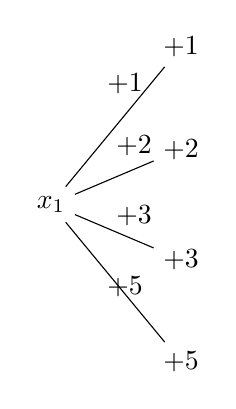
\begin{tikzpicture}
			\path node (x1) {$x_1$};
			\path (x1.east) ++ (\DUNodeSep, 20mm) node[anchor=west] (c11) {\DBval{+1}};
			\path (x1.east) ++ (\DUNodeSep, 7mm) node[anchor=west] (c12) {\DBval{+2}};
			\path (x1.east) ++ (\DUNodeSep, -7mm) node[anchor=west] (c13) {\DBval{+3}};
			\path (x1.east) ++ (\DUNodeSep, -20mm) node[anchor=west] (c14) {\DBval{+5}};
			\path[draw] (x1) -- (c11) node[pos=0.6, shift={(0, 4mm)}] {\SI{+1}{\degreeCelsius}};
			\path[draw] (x1) -- (c12) node[pos=0.75, shift={(0, 3mm)}] {\SI{+2}{\degreeCelsius}};
			\path[draw] (x1) -- (c13) node[pos=0.75, shift={(0, 3mm)}] {\SI{+3}{\degreeCelsius}};
			\path[draw] (x1) -- (c14) node[pos=0.6, shift={(0, 1mm)}] {\SI{+5}{\degreeCelsius}};
		\end{tikzpicture}
		\setcounter{DBxc}{2}
		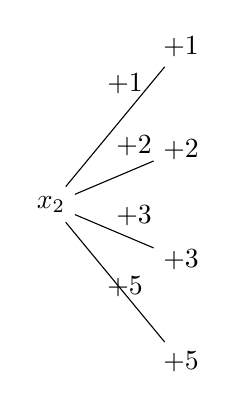
\begin{tikzpicture}
			\path node (x1) {$x_2$};
			\path (x1.east) ++ (\DUNodeSep, 20mm) node[anchor=west] (c11) {\DBval{+1}};
			\path (x1.east) ++ (\DUNodeSep, 7mm) node[anchor=west] (c12) {\DBval{+2}};
			\path (x1.east) ++ (\DUNodeSep, -7mm) node[anchor=west] (c13) {\DBval{+3}};
			\path (x1.east) ++ (\DUNodeSep, -20mm) node[anchor=west] (c14) {\DBval{+5}};
			\path[draw] (x1) -- (c11) node[pos=0.6, shift={(0, 4mm)}] {\SI{+1}{\degreeCelsius}};
			\path[draw] (x1) -- (c12) node[pos=0.75, shift={(0, 3mm)}] {\SI{+2}{\degreeCelsius}};
			\path[draw] (x1) -- (c13) node[pos=0.75, shift={(0, 3mm)}] {\SI{+3}{\degreeCelsius}};
			\path[draw] (x1) -- (c14) node[pos=0.6, shift={(0, 1mm)}] {\SI{+5}{\degreeCelsius}};
		\end{tikzpicture}
	\end{exampleblock}
	$R$ indicates whether $x_1$ is preferred to $x_2$, …
\end{frame}

\begin{frame}
	\frametitle{Decision under risk}
	\begin{itemize}
		\item “Risk” used when probabilities are known
		\item Probability measure $p$ over the powerset of $S$
		\item $p(s) \in [0, 1]$ (with $s \subseteq S$): probability of occurence of $s$, $p(S) = 1$
	\end{itemize}
	\begin{exampleblock}{Moving production: with probabilities}
		$p(\SI{+1}{\degreeCelsius}) = 0.2; p(\SI{+2}{\degreeCelsius}) = 0.1; p(\SI{+3}{\degreeCelsius})=0.4; p(\SI{+5}{\degreeCelsius})=0.3$
		\centering
		\setlength{\DUNodeSep}{1cm}
		\setcounter{DBxc}{1}
		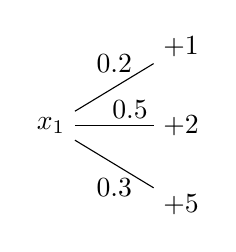
\begin{tikzpicture}
			\path node (x1) {$x_1$};
			\path (x1.east) ++ (\DUNodeSep, 10mm) node[anchor=west] (c11) {\DBval{+1}};
			\path (x1.east) ++ (\DUNodeSep, 0mm) node[anchor=west] (c12) {\DBval{+2}};
			\path (x1.east) ++ (\DUNodeSep, -10mm) node[anchor=west] (c14) {\DBval{+5}};
			\path[draw] (x1) -- (c11) node[pos=0.5, yshift=3mm] {\num{0.2}};
			\path[draw] (x1) -- (c12) node[pos=0.5, shift={(2mm, 2mm)}] {\num{0.5}};
			\path[draw] (x1) -- (c14) node[pos=0.5, shift={(0, -3mm)}] {\num{0.3}};
		\end{tikzpicture}
		\setcounter{DBxc}{2}
		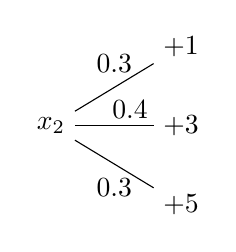
\begin{tikzpicture}
			\path node (x1) {$x_2$};
			\path (x1.east) ++ (\DUNodeSep, 10mm) node[anchor=west] (c11) {\DBval{+1}};
			\path (x1.east) ++ (\DUNodeSep, 0mm) node[anchor=west] (c12) {\DBval{+3}};
			\path (x1.east) ++ (\DUNodeSep, -10mm) node[anchor=west] (c14) {\DBval{+5}};
			\path[draw] (x1) -- (c11) node[pos=0.5, yshift=3mm] {\num{0.3}};
			\path[draw] (x1) -- (c12) node[pos=0.5, shift={(2mm, 2mm)}] {\num{0.4}};
			\path[draw] (x1) -- (c14) node[pos=0.5, shift={(0, -3mm)}] {\num{0.3}};
		\end{tikzpicture}
	\end{exampleblock}
\end{frame}

\begin{frame}
	\frametitle{Decision under risk: comparing probabilities}
	$x \in \allalts$ can be viewed as a probability mass $p_x: C → [0, 1]$ over the consequences.
	\begin{exampleblock}{Moving production: comparing probabilities}
		\centering
		\setlength{\DUNodeSep}{0mm}
		\setcounter{DBxc}{1}
		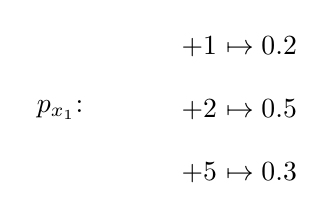
\begin{tikzpicture}
			\path node (p1) {$p_{x_1}$:};
			\path (p1.east) ++ (\DUNodeSep, 8mm) node[anchor=west] (c11) {\DBval{+1} $\mapsto \num{0.2}$};
			\path (p1.east) ++ (\DUNodeSep, 0mm) node[anchor=west] (c12) {\DBval{+2} $\mapsto \num{0.5}$};
			\path (p1.east) ++ (\DUNodeSep, -8mm) node[anchor=west] (c14) {\DBval{+5} $\mapsto \num{0.3}$};
		\end{tikzpicture}
		\setcounter{DBxc}{2}
		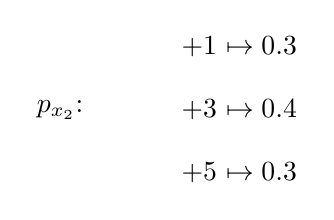
\begin{tikzpicture}
			\path node (p1) {$p_{x_2}$:};
			\path (p1.east) ++ (\DUNodeSep, 8mm) node[anchor=west] (c11) {\DBval{+1} $\mapsto \num{0.3}$};
			\path (p1.east) ++ (\DUNodeSep, 0mm) node[anchor=west] (c12) {\DBval{+3} $\mapsto \num{0.4}$};
			\path (p1.east) ++ (\DUNodeSep, -8mm) node[anchor=west] (c14) {\DBval{+5} $\mapsto \num{0.3}$};
		\end{tikzpicture}
	\end{exampleblock}
	\begin{itemize}
		\item Alternative also called a \emph{lottery}
		\item $R$ indicates whether $p_{x_1}$ is preferred to $p_{x_2}$, …
	\end{itemize}
\end{frame}

\begin{frame}
	\frametitle{Weak order}
	\begin{definition}[Weak order]
		$\succeq$ is a \emph{weak order} iff it is:
		\begin{description}[Connected]
			\item[Transitive] $x \succeq y \succeq z ⇒ x \succeq z$
			\item[Connected] $\forall x ≠ y$, $x \succeq y$ or $y \succeq x$
	%		\item[Antisymmetric] $\forall a ≠ b$, only one of $a \succeq b$ or $b \succeq a$
			\item[Reflexive] $x \succeq x$
		\end{description}
	\end{definition}
	\begin{itemize}
		\item Complete ⇔ connected and reflexive
%		\item Can $\succeq$ admit cycles? \onslide<2->{Yes, in an equivalence class}
%		\item Is $≥$ in $\R$ a weak order? \onslide<3->{Yes, with no ex-æquo}
%		\item Is $>$ in $\R$ a weak order? \onslide<4>{No: not reflexive}
		\item $\succeq$ defines ordered equivalence classes
	\end{itemize}
\end{frame}

\begin{frame}
	\frametitle{Numerical representation of a weak order}
	\begin{theorem}[Weak order and utility \citep{fishburn_utility_1970}]
		Given a binary relation $\succeq$ on a set $\allalts$, assume $\allalts$ is finite. Then, these two conditions are equivalent.
		\begin{itemize}
			\item $\succeq$ is a weak order
			\item There exists a $u: \allalts → \R$ such that
			\begin{equation}
				\tag{$u$ represents $\succeq$}
				u(x) ≥ u(y) ⇔ x \succeq y
			\end{equation}
		\end{itemize}
	\end{theorem}
	(Citations do \emph{not} indicate paternity.)
	\begin{itemize}
		\item The theorem goes through with $\allalts$ infinite and $(\allalts, \succeq)$ satisfying some denseness condition
		\item $u$ is called a \emph{utility} (or \emph{value}) function
	\end{itemize}
\end{frame}

\begin{frame}
	\frametitle{Significance of the scale}
	Any increasing transformation of $u$ also represents $\succeq$
	\begin{itemize}
		\item If $u$ represents $\succeq$
		\item Define $u' = t \circ u$ with $r ≤ s ⇒ t(r) ≤ t(s)$
		\item Then $u'$ also represents $\succeq$
	\end{itemize}
	\begin{exampleblock}{Equivalent utility functions}
		\centering
		\begin{tikzpicture}
			\path node (x) {$x$};
			\path (x) ++ (3mm, 6mm) node (y) {$y$};
			\path node[fit={(x) (y)}, circle, draw, inner sep=0] (set) {};
			\path (set.north west) node[anchor=south east] (X) {$\allalts$};
			\path (set.south) ++ (0, -3mm) coordinate (bottom set);
			\path (set.north) ++ (0, 5mm) coordinate (top set);
			\path (bottom set) ++ (30mm, 0) coordinate (bottom u) ++(0, 3mm) coordinate (2 u) ++(0, 4mm) coordinate (3 u) ++(0, 4mm) coordinate (4 u) ++(0, 4mm) coordinate (5 u) ++(0, 4mm) coordinate (6 u);
			\path (top set -| bottom u) coordinate (top u);
			\path[draw] (bottom u) --plot[mark=+]  coordinates{(3 u) (4 u)} [->] -- (top u);
			\path (3 u.east) node[anchor=east] (3 u figure) {$3$};
			\path (4 u.east) node[anchor=east] (4 u figure) {$4$};
			\path (bottom u) ++ (30mm, 0) coordinate (bottom u');
			\path (bottom u' |- 2 u) coordinate (2 u') node[anchor=west] {$2$};
			\path (bottom u' |- 6 u) coordinate (6 u') node[anchor=west] {$6$};
			\path (bottom u' |- top u) coordinate (top u');
			\path[draw] (bottom u') --plot[mark=+]  coordinates{(2 u') (6 u')} [->] -- (top u');
			\path[draw, ->] (x) -- (3 u figure);
			\path[draw, ->] (y) -- (4 u figure);
			\path[draw, ->] ($(3 u)!2mm!(2 u')$) -- ($(2 u')!2mm!(3 u)$);
			\path[draw, ->] ($(4 u)!2mm!(6 u')$) -- ($(6 u')!2mm!(4 u)$);
			\path (top set) ++(0, 1mm) [draw, ->] to[bend left=30] node[shift={(0, 2mm)}] {$u$} ($(top u)+(-1mm, 1mm)$);
			\path (top u) ++(1mm, 1mm) [draw, ->] to[bend left=30] node[shift={(0, 2mm)}] {$t$} ($(top u')+(-1mm, 1mm)$);
			\path (bottom set) ++(0, -1mm) [draw, ->] to[bend left=-20] node[shift={(0, 2mm)}] {$u'$} ($(bottom u')+(-1mm, -1mm)$);
		\end{tikzpicture}
	\end{exampleblock}
\end{frame}

\begin{frame}
	\frametitle{Numerics and risk}
	Consider a context of decision under risk.
	\begin{theorem}
%		\setlength\abovedisplayskip{1 ex}% reduce space above equations
		$\succeq$ satisfies:
		\begin{description}[Independence]
			\item[Order] $\succeq$ is a weak order
			\item[Independence] Given $x \succeq y$, any $z \in \allalts$, and $0 < \alpha < 1$: $\alpha p_x + (1 − \alpha) p_z \succeq \alpha p_y + (1 − \alpha) p_z$
			\item[Continuity] Given $x \succeq y \succeq z$, for some $0 < \alpha, \beta < 1$: $\alpha p_x + (1 − \alpha) p_z \succeq p_y \succeq \beta p_x + (1 − \beta) p_z$
		\end{description}
		iff $\exists u: \allalts → \R$ and $u': C → \R$ such that
		\begin{equation}
			\tag{$u$ represents $\succeq$}
			u(x) ≥ u(y) ⇔ x \succeq y,
		\end{equation}
%		and
		\begin{equation}
			\tag{$u$ is an expectation}
			u(x) = \sum_c u'(c) p_x(c).
		\end{equation}
	\end{theorem}
\end{frame}

\begin{frame}
	\frametitle{Numerics and risk: comments}
	\begin{itemize}
		\item $u$ is now determined up to affine transformations only
		\item $u(p_c) = u'(c)$, with $p_c$ being $c$ with probability one
	\end{itemize}
\end{frame}

\section[Reasons]{Reasons for incomplete models}
\begin{frame}
	\frametitle{Two interpretations of incomplete models}
	\begin{itemize}
		\item Epistemic incompleteness: incomplete model because the modeler ignores parts of it
		\item Ontologic incompleteness: incomplete model even when the modeler knows everything
	\end{itemize}
	I will talk about \emph{ontological} incompleteness
\end{frame}

\begin{frame}
	\frametitle{Arguments for ontological incompleteness}
	\begin{description}[Epistemological]
		\item[Epistemological] A better representation of reality
		\item[Ethical] May permit to give better grounded recommandations (avoid recommending debatable behavior)
		\item[Practical] Useful for building consensus in group decision making
	\end{description}
	Disclaimer: this part presents personal opinions
\end{frame}

\subsection{Epistemological}
\begin{frame}
	\frametitle{Rebutting completeness}
	Completeness sometimes considered true by definition.
	\begin{block}{An argument for completeness}
		Offer the choice between two alternatives. The user picks either $x$ or $y$ or is indifferent. Iterate. Obtain a complete model.
	\end{block}
	This argument has two weaknesses
	\begin{enumerate}
		\item We might want to study (more) \emph{stable} preference
		\item We might want to model (more) \emph{reflexive} preference
	\end{enumerate}
\end{frame}

\begin{frame}
	\frametitle{Local VS stable preferences}
	\begin{itemize}
		\item Argument for completeness considers “preference” as a set of time- and place- located events
		\item What if we are interested in her stable preference over some time span?
	\end{itemize}
	\begin{block}{\citet{tversky_intransitivity_1969} on incompleteness of stable preferences}
		\begin{itemize}
			\item Users “are not perfectly consistent in their choices”
			\item “often choose $x$ in some instances and $y$ in others”
			\item Inconsistencies observed “even in the absence of systematic changes in (…) taste (…) due to learning or sequential effects”
			\item Inconsistencies thus seem to “reflect inherent variability or momentary fluctuation in the evaluative process”
		\end{itemize}
	\end{block}
\end{frame}

\begin{frame}
	\frametitle{Intuitive preference}
	von Neumann and Morgenstern (vNM) use a notion of “intuitive” preference
	\begin{block}{Preference in the vNM sense \citep{fishburn_retrospective_1989}}
		The “immediate sensation of preference” provides the basis for the measurement of utility
	\end{block}
	\begin{block}{Completeness in the vNM sense}
		For any two objects, the user “possesses a clear intuition of preference”. “[W]e expect him, for any two [alternatives] which are put before him as possibilities, to be able to tell which of the two he prefers”.
	\end{block}
\end{frame}

\begin{frame}
	\frametitle{Arguments for reflexive preference}
	Reflexive preference: those you stick to after having thought about it
	\begin{itemize}
		\item When recommending, we want to help decide
		\item Protection against (obvious) “bad behavior” might be useful
		\item Is the recommendation system falling under manipulative actions by vendors?
		\item Intuitive preference is not transitive \citep{mandler_difficult_2001}
	\end{itemize}
\end{frame}

\subsection{Ethical}
\begin{frame}
	\frametitle{Ethical argument for incomplete models}
	\begin{itemize}
		\item Can we assume that preferences are complete as an approximation?
		\item Psychology shows that intuitive behavior can be non reflexive
		\item Ethical argument: recommendation systems may protect against (worst forms of) such behavior
		\item Does not apply to all recommendation systems!
	\end{itemize}
\end{frame}

\begin{frame}
	\frametitle{Experimental psychology and MCDA}
	An example of effects known in experimental psychology
	\begin{itemize}
		\item Two criteria
		\item Ask questions to obtain preference model $R$
		\item Assume $R$ satisfies dominance and transitivity
		\item Trade-offs differ depending on the way questions are asked
		\item By choosing the kind of questioning strategy, you choose whether to accentuate the most salient criterion
	\end{itemize}
\end{frame}

\begin{frame}
	\frametitle{Two kinds of trade-off questions}
	\begin{block}{Binary choice}
		Choose one alternative
		\begin{center}
			\begin{tabular}{lrrl}
					& Price	& Distance from center\\
				\hline
				Hotel $a$	& 86	& 16\\
				Hotel $b$	& 68	& 31\\
				\hline
			\end{tabular}
		\end{center}
	\end{block}
	\begin{block}{Matching}
		Make the alternatives equally attractive
		\begin{center}
			\begin{tabular}{lrrl}
					& Price	& Distance from center\\
				\hline
				Hotel $x$	& 86	& 16\\
				Hotel $y$	& ?	& 31\\
				\hline
			\end{tabular}
		\end{center}
		Then we deduce whether $a=(86, 16) \succeq b=(68, 31)$.
	\end{block}
\end{frame}

\begin{frame}
	\frametitle{Experimental psychology and decision under risk}
	\begin{itemize}
		\item Similar effects exist under the “risk” context
		\item Ask using probability equivalents: Prefer $p_x = (0.5, 10 VS 0)$ to $p_y = (?, 20 VS 0)$?
		\item Or ask using certainty equivalents: Prefer $p_x = (0.5, 10 VS 0)$ to $p_y = (1, ?)$?
	\end{itemize}
\end{frame}

\begin{frame}
	\frametitle{Remarks about preference reversal effects}
	\begin{itemize}
		\item Effects called preference reversal (by procedure or description variance)
		\item Existence of those effects is consensual
		\item Interpretation is not
		\item Psychologist’s conclusion: frame must be fixed
		\item Other possible conclusion: reflexive preferences may be incomplete
		\item More research needed
	\end{itemize}
\end{frame}

\subsection{Practical}
\begin{frame}
	\frametitle{Practical argument for incomplete models}
	\begin{itemize}
		\item The model may reflect what’s truly preferable for the user
		\item The model may have more degrees of freedom
	\end{itemize}
	\begin{block}{Illustration: group decision making}
		\begin{itemize}
			\item In group decision approach: more possibilities for consensus
			\item Build a second model lexicographically
			\item First order: what the user prefers for intrinsic reasons
			\item Second order: what the user allows for reasons of being nice to others, …
		\end{itemize}
	\end{block}
\end{frame}

\section{Means}
\begin{frame}
	\frametitle{In this subsection}
	\begin{itemize}
		\item Outranking approach
		\item (More) classical economists / psychologists approach
	\end{itemize}
	Disclaimer: more research needed for application to recommender systems!
\end{frame}

\subsection{Outranking approach}
\begin{frame}
	\frametitle{Outranking approach}
	\begin{itemize}
		\item Context: MCDM
		\item Outranking approach is an alternative to value (utility) theory
		\item Relaxes assumptions
		\item Intuition 1: compare alternatives pairwise
		\item Intuition 2: several points of view may conflict
		\item From \emph{one} POV, $x$ is better than $y$
	\end{itemize}
\end{frame}

\begin{frame}
	\frametitle{Illustration with Electre III}
	(Method is much simplified here)
	\begin{itemize}
		\item General idea: build two relations $C, D$
		\item Define $x {\mathrel{R}} y ⇔ x {\mathrel{C}} y \text{ and not } x {\mathrel{D}} y$
		\item $C$ for concordance: reasons in favor
		\item $D$ for discordance: reasons against
		\item $x \mathrel{C} y$ iff $x$ is sufficiently better than $y$ for being preferred
		\item For $C$, only criteria in favor of $x$ are considered
		\item $x \mathrel{D} y$ iff some strong reasons oppose $x$ being preferred to $y$
		\item $D$ only looks for reasons against
	\end{itemize}
\end{frame}

\begin{frame}
	\frametitle{Example}
%	\begin{block}{Parameters of the model}
%		\begin{itemize}
%			\item Weights $w_\crit \in [0,1], {\crit \in \crits}, \sum_\crit w_\crit = 1$
%			\item Threshold $\lambda \in [0.5, 1]$
%			\item Veto thresholds $\v_\crit \in \R$ (assuming $X_\crit \subseteq \R$)
%		\end{itemize}
%	\end{block}
	\begin{exampleblock}{Example relations}
		\begin{itemize}
			\item $x C y$ iff $x$ is better than $y$ (or equal) for at least two criteria
			\item $x D y$ iff $\exists \crit \in \crits \suchthat y_g - x_g ≥ 3$
		\end{itemize}
	\end{exampleblock}
	\begin{center}
		\begin{tikzpicture}
			\path node[matrix of nodes, ampersand replacement=\&] (my matrix) {
					\& quantity	\& taste	\& \node[align=left] {resists\\to cold};\\
				Tomatoes	\& 4	\& 4	\& | (st 1) | 1\\
				Cabbage	\& 4	\& 1	\& | (st 3) | 5\\
				Potatoes	\& 2	\& 2	\& | (st 4) | 4\\
			};
		\end{tikzpicture}
	\end{center}
	\vspace{-1em}
	\begin{itemize}
		\item Cabbage $\succeq$ Potatoes
		\item Tomatoes incomparable to Cabbage and Potatoes
	\end{itemize}
\end{frame}

\subsection{Semiorders}
\begin{frame}
	\frametitle{Another case of incomparability}
	\begin{itemize}
		\item $x$ indistingushable to $y$ and $y$ to $z$
		\item But $x \succeq z$
		\item Luce’s “grain of sugar”
		\item How to represent this numerically?
		\item Which kinds of structure does this correspond to?
	\end{itemize}
\end{frame}

\begin{frame}
	\frametitle{Semiorder}
	\begin{definition}[Semiorder \citep{fishburn_utility_1970}]
		A binary relation $R$ is a \emph{semiorder} iff it is irreflexive, transitive, and satisfies C1 and C2
%		\begin{itemize}
%			\item Irreflexive
%			\item Transitive
%			\item C1
%			\item C2
%		\end{itemize}
	\end{definition}
	\begin{block}{C1}
		\begin{tikzpicture}[baseline=($(x.south)!0.75!(y.north)$)]
			\path node (x) {$x$};
			\path (x.south) ++(0, -\GraphsNodeSep) node[anchor=north] (y) {$y$};
			\path (x.base east) ++(1em, 0) node[anchor=base west] (z) {$z$};
			\path (y.base east) ++(1em, 0) node[anchor=base west] (w) {$w$};
			\path ($(x.base east)!0.5!(z.base west)$) node[anchor=base] {$\sim$};
			\path ($(y.base east)!0.5!(w.base west)$) node[anchor=base] {$\sim$};
			\path[draw] (x) -- (y);
			\path[draw] (z) -- (w);
		\end{tikzpicture}
		$⇒$
		\begin{tikzpicture}[baseline=($(x.south)!0.75!(y.north)$)]
			\path node (x) {$x$};
			\path (x.south) ++(0, -\GraphsNodeSep) node[anchor=north] (y) {$y$};
			\path (x.base east) ++(1em, 0) node[anchor=base west] (z) {$z$};
			\path (y.base east) ++(1em, 0) node[anchor=base west] (w) {$w$};
			\path[draw] (x) -- (w);
		\end{tikzpicture}
		or
		\begin{tikzpicture}[baseline=($(x.south)!0.75!(y.north)$)]
			\path node (x) {$x$};
			\path (x.south) ++(0, -\GraphsNodeSep) node[anchor=north] (y) {$y$};
			\path (x.base east) ++(1em, 0) node[anchor=base west] (z) {$z$};
			\path (y.base east) ++(1em, 0) node[anchor=base west] (w) {$w$};
			\path[draw] (z) -- (y);
		\end{tikzpicture}
	\end{block}
	\begin{block}{C2}
		\begin{tikzpicture}[baseline=(current bounding box.center)]
			\path node (x) {$x$};
			\path (x.south) ++(0, -\GraphsNodeSep) node[anchor=north] (y) {$y$};
			\path (y.south) ++(0, -\GraphsNodeSep) node[anchor=north] (z) {$z$};
			\path (y.base east) ++(1em, 0) node[anchor=base west] (w) {$w$};
			\path ($(y.base east)!0.5!(w.base west)$) node[anchor=base] {$\sim$};
			\path[draw] (x) -- (y);
			\path[draw] (y) -- (z);
		\end{tikzpicture}
		$⇒$
		\begin{tikzpicture}[baseline=(current bounding box.center)]
			\path node (x) {$x$};
			\path (x.south) ++(0, -\GraphsNodeSep) node[anchor=north] (y) {$y$};
			\path (y.south) ++(0, -\GraphsNodeSep) node[anchor=north] (z) {$z$};
			\path (y.base east) ++(1em, 0) node[anchor=base west] (w) {$w$};
			\path[draw] (x) -- (w);
		\end{tikzpicture}
		or
		\begin{tikzpicture}[baseline=(current bounding box.center)]
			\path node (x) {$x$};
			\path (x.south) ++(0, -\GraphsNodeSep) node[anchor=north] (y) {$y$};
			\path (y.south) ++(0, -\GraphsNodeSep) node[anchor=north] (z) {$z$};
			\path (y.base east) ++(1em, 0) node[anchor=base west] (w) {$w$};
			\path[draw] (w) -- (z);
		\end{tikzpicture}
		\vspace{-0.4pt}
	\end{block}
\end{frame}

\begin{frame}
	\frametitle{Representation}
	\begin{theorem}[\citealt{luce_semiorders_1956,scott_foundational_1958}]
		Given a semiorder $R$ on $\allalts$ finite, there exists $u: \allalts → \R$ such that:
		\begin{equation}
			x R y ⇔ u(x) + 1 < u(y)
		\end{equation}
	\end{theorem}
	\vspace{1em}
	Example incomparability:
	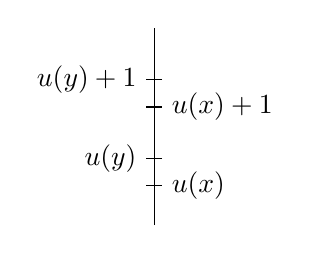
\begin{tikzpicture}[baseline=(current bounding box.center)]
		\path[draw] (0, 0.5) -- (0, 3);
		\path[draw] (-0.1, 1) -- (0.1, 1) node[anchor=west] (ux) {$u(x)$};
		\path[draw] (0.1, 1.35) -- (-0.1, 1.35) node[anchor=east] (ux) {$u(y)$};
		\path[draw] (-0.1, 2) -- (0.1, 2) node[anchor=west] {$u(x) + 1$};
		\path[draw] (0.1, 2.35) -- (-0.1, 2.35) node[anchor=east] {$u(y) + 1$};
	\end{tikzpicture}
\end{frame}

\section[Conclusion]{Conclusion and further remarks}
\subsection{Norms and models}
\begin{frame}
	\frametitle{A normative property of decision}
	If you prefer $x$ to $y$, you ought to not reverse your preference in presence of $z$ (says the normative property)
	\begin{block}{Counter-example}
		\begin{itemize}
			\item “Would you like chocolate cake or coconut cake?”
			\item “I prefer the chocolate cake!”
			\item “Oh, by the way, there’s also ice cream”
			\item “Mmh, give me the coconut cake”
		\end{itemize}
	\end{block}
	Odd?
\end{frame}

\begin{frame}
	\frametitle{Sen on the act of choice}
	\begin{itemize}
		\item \citet{sen_maximization_1997} warns against too simple usage of this norm
		\item You are invited at a garden party
		\item Out of {apple, banana}, you would pick apple
		\item Out of {apple, mango, banana}, you would pick banana
	\end{itemize}
	Possible explanation? \pause
	\begin{itemize}
		\item You prefer mango to banana to apple
		\item You suspect everyone else has the same preference
		\item You want to be polite and take the second best
	\end{itemize}
	⇒ Reasonableness of norms are relative to a model
\end{frame}

\subsection{Conclusion}
\begin{frame}
	\frametitle{Conclusion}
	\begin{itemize}
		\item Movie recommendation system that predicts [1, 5] stars: might be less determined than usually believed?
		\item More research needed!
		\item Pay attention to the model
		\item Majority of the literature is about complete models; but more and more analysis about incompleteness
		\item My interpretation may not be consensual! (But the displayed knowledge is)
		\item There are also valid reasons for complete models (but think about it!)
	\end{itemize}
\end{frame}

\begin{frame}[plain]
	\addtocounter{framenumber}{-1}
	\begin{center}
		\huge
		\textit{Thank you for your attention!}
	\end{center}
\end{frame}

\appendix
\AtBeginSection{
}

\clearpage\pdfbookmark[2]{\refname}{\refname}
\begin{frame}[allowframebreaks]
	\frametitle{\refname}
 	\bibliography{Survey}
\end{frame}

\clearpage\pdfbookmark{License}{License}
\begin{frame}[plain]
	\frametitle{License}
	This presentation, and the associated \LaTeX{} code, are published under the \href{http://opensource.org/licenses/MIT}{MIT license}. Feel free to reuse (parts of) the presentation, under condition that you cite the author.
	
	Credits are to be given to \href{http://www.lamsade.dauphine.fr/~ocailloux/}{Olivier Cailloux}, Université Paris-Dauphine.
\end{frame}
\addtocounter{framenumber}{-1}
\end{document}

\begin{frame}
	\frametitle{\subsecname}
	\begin{itemize}
		\item 
	\end{itemize}
\end{frame}

